\documentclass[conference]{IEEEtran}

%\usepackage[russian]{babel}
\usepackage[justification=centering]{caption}
\usepackage[backend=bibtex,sorting=none]{biblatex}
\usepackage{fontspec}
\usepackage[final]{graphicx}
\usepackage{tabularx,booktabs}
\newcolumntype{C}{>{\centering\arraybackslash}X} % centered version of "X" type
\setlength{\extrarowheight}{3pt}
\usepackage{float}
\usepackage{subcaption}
\usepackage{adjustbox}
\usepackage{listings}
\usepackage{array}
\usepackage{xcolor}
\usepackage{graphicx}
\usepackage{tikz}
\usepackage{pgfplots}
%\usepackage{geometry}
\graphicspath{{./images/}}

\setmainfont{Spectral Light}%{Times New Roman}

\definecolor{codegreen}{rgb}{0,0.6,0}
\definecolor{codegray}{rgb}{0.5,0.5,0.5}
\definecolor{codepurple}{rgb}{0.58,0,0.82}
\definecolor{backcolour}{rgb}{0.95,0.95,0.92}

\lstdefinestyle{mystyle}{
    backgroundcolor=\color{white},   
    commentstyle=\color{codegreen},
    keywordstyle=\color{magenta},
    numberstyle=\color{codegray},
    stringstyle=\color{codepurple},
    basicstyle=\ttfamily\footnotesize,
    morekeywords={*,procedure, if, rol, cmpj, setmask, then, else, endif, cmpjn, is, not, and, return},            % if you want to add more keywords to the set
    breakatwhitespace=false,         
    breaklines=true,                 
    captionpos=b,                    
    keepspaces=true,                 
    numbers=left,                    
    numbersep=10pt,
    xleftmargin=7mm,
    xrightmargin=0mm,
    showspaces=false,                
    showstringspaces=false,
    showtabs=false,                  
    tabsize=4
}
\lstset{style=mystyle}
\lstset{linewidth=9cm}
\bibliography{syrcose} 


\begin{document}
\author{
    \IEEEauthorblockN{Nikita Nikiforov}
    \IEEEauthorblockA{\textit{Lomonosov Moscow State University}\\
    Moscow, Russia\\
    nickiforov.nik@gmail.com}
    \and
    \IEEEauthorblockN{Dmitry Volkanov}
    \IEEEauthorblockA{\textit{Lomonosov Moscow State University}\\
    Moscow, Russia\\
    volkanov@asvk.cs.msu.ru}
    }
\title{
    Data compression algorithms for flow tables in Network Processor RuNPU.
}
\maketitle
    \begin{abstract}
        This   paper   addresses   the   problem   of   packet classification  within  a  network  processor  (NP)  
        architecture without the separate associative device. By the classification, we  mean  the  process  of  
        identifying  a  packet  by  its  header.The classification stage requires the implementation of data 
        structures  to  store  the  flow  tables.  In  our  work  we  consider the  NP  without  the  associative  memory.  
        Flow  tables  are represented by an assembly language program in the NP. For translating  flow  tables  into  assembly  
        language  programs,  a tables translator was used. The main reason for implementing data  compression  algorithms  in  a  
        flow  tables  translator  is that  modern  flow  tables  can  take  up  to  tens  of  megabytes. In  this  paper  we  
        describe  the  following  data  compression algorithms: Optimal rule caching, recursive end-point cutting and common data compression algorithms. 
        An evaluation of the implemented data compression algorithms was performed on a simulation model of the NP.
    \end{abstract}
    
    \begin{IEEEkeywords}
        Network processor, software-defined networks, packet classification, data compression.
    \end{IEEEkeywords}

    \section{Introduction}
        At present, software-defined networks (SDN) are in active development and require high-performance switches~\cite{smel2012open}.
        The main functional element of the high-performance SDN switch is a programmable network processor (NP). 
        The network processor is a system-on-chip specialized for network packet processing. 
        In this work we consider a programmable NP. A programmable NP is one that supports on-the-fly modification of the packet 
        processing program and the set of header fields to be processed. 

        In this article we discuss data compression algorithms used for flow tables. Flow tables are needed for packet classification process. 
        A flow table is the set of rules defined by OpenFlow protocol. OpenFlow is one of the most common protocols 
        for controlling a network SDN switch. This paper considers OpenFlow version 1.3~\cite{openflow}. Each rule contains a match field, 
        a bit string by witch a packet can be identified and a set of actions, that the NP performs on this packet. 
        Classification is the process of the identification of a network packet by its header.

        This article has the following structure: in second section we introduce problem, in third section we introduce 
        the NP architecture and flow tables translator, in fourth section we describe related work, in fifth section we
        describe data compression algorithm implementation and in sixth section we introduce our evaluation methodology.

    \section{The problem}
    \label{sect:problem}
        Let us consider OpenFlow tables formalisation. An ordered set of all considered attributes is denoted as \(I=\{m_1,m_2,\ldots,m_k\}\). 
        Every attribute \(m_i\) from the set \(I\) is described by a bit string \(m_i \in \{0, 1, *\}^W_i\).
        In this article symbol \(*\) denotes any bit. But, if \(\exists m_i^j \in m_i\) and  \( m_i^j = *\), 
        then for \( \forall m_i^k \), where \(k > j\), \( m_i^k = *\). The length of the attribute is denoted \(len(m_i) = W_i\).

        Flow tables are represented by a set of rules \(R=\{r_1,r_2,\ldots,r_n\}\). With every rule \(r_i\) binding the features:
        \begin{itemize}
            \item An index \(i\);
            \item A priority \(p_i \in Z_+\);
            \item A vector of values of attributes \(f_i=\{f_i^1,f_i^2,\ldots,f_i^k\}\), where \(f_i^j\) is an attribute value \(m_j\in I\). % и \(f_i^j\in D(m_j)\cup\{*\}\), \(j=\overline{1,k}\).
            \item A set of actions \(A_i = \{a_1, a_2, \ldots, a_z\} \).
        \end{itemize}

        A network packet header \(x\) and its metadata with vector values of attributes \(g=\{g^1,g^2,\ldots,g^k\}\) (\(x \rightarrow g\)),
        a match rule \(r_i\in R\) with a vector of values of the attributes \(f_i=\{f_i^1,f_i^2,\ldots,f_i^k\}\) 
        and a priority \(p_i\) (a rule \(r_i\in R\) identifies a network packer with a vector values of attributes \(g\)), if:

        \begin{enumerate}
            \item a vector values of attributes \(g\) match a vector of values of the attributes \(f_i\), 
                \(\forall g_i \in g\), \(len(g_i) = len(f_i)\). \(\forall f_i^{lj} \in f_i^l\), \(f_i^{lj} \in \{*, g^{lj}\}\), \(l=\overline{1,k}\);
            \item a priority \(p_i\) is the highest among all rules \(r_j\in R\), if a vector \(g\) match a vector\(f_j\).
        \end{enumerate}

        The set of rules \(R\) must satisfy the following constraint. 
        For any two rules \(r_i,r_j\in R,r_i\not= r_j\),  if their vectors of values intersect, there is a set of attribute values. 
        This set corresponds to vectors of values of attributes of both rules  \(p_i\not= p_j\). 
        
        Let us introduce the function for network packet identification \(x \rightarrow g\)in flow table \(R\), (denotes as \(R(x)\)).
        It returns a set of actions, that corresponded to the rule \(x \rightarrow g\). 
        \begin{center}
            \(R(x) = A_{r_i}\), where \(A_{r_i}\) is the set of actions \(r_i \in R\).
        \end{center}

        We need to introduce a {\bf similar concept} of the sets of rules \(R_1\) and \(R_2\).
        The set \(R_1\) is similar to the set \(R_2\), when for any network packet header, 
        that can be identified by some rule from the set \(r_i \in R_1\),
        and there exists another rule that identifies it as \(r_j \in R_2\), and \(A_i = A_j\).

        We need to develop an algorithm for compressing flow tables. This algorithm must translate an input flow table (a set of rules \(R_1\))
        into a new compressed set of rules \(R_2\). 
        \begin{enumerate}
            \item The set of rules \(R_1\) is similar to the set of rules \(R_2\).
            \item The cardinality of the set \(R_2\) must be lower than the cardinality of the set \(R_1\).
        \end{enumerate}
    
    \section{Network processor architecture}
            \label{section:problem}
        In the considered NP the pipeline architecture is used, with each pipeline consisting of 10 computing blocks. 
        To avoid complex memory organization, there is no associative memory in the considered NP. 
        The NP uses the same memory both for commands and data.
         
        Let us consider the pipeline NP architecture. 
        Each computing block has an access to the memory area where the program with data is located.
        There is a limit of 25 clock cycles per packet on each processing block.
        There is up to 512 kilobytes to store assembly language program representing flow tables.
        Due to the instruction set architecture, there is no separate memory area where data is stored. 
        Therefore, the microcode contains all the data, required to classify packets.
        
        \subsection{Flow tables translator}
            Flow tables translator is a tool that is executed on CPU. It is used for flow tables translating
            into assembly language programs, that can be interpreted by NP. Flow tables translator uses 
            tree structures for flow table representation.
            Every node of the tree structure can be associated with a table rule. 
            After building a tree every node is translated into a part of an assembly
            language program. Here is a flow tables translator workflow:
            \begin{enumerate}
                \item Load a flow table from file.
                \item Check every rule in the table.
                \item Build a tree structure from a set of rules.
                \item Translate every node into a part of an assembly language program.
                \item Combine all translated parts into the one assembly language program.
                \item Add a header that corresponds to used protocol.
                \item Write the assembly language program into file.
            \end{enumerate}

            This tool was implemented in work~\cite{andrewmonetec}.

    \section{Related work}
        In this section we  introduce a review on data compression algorithms, that already used
        for other network processors~\cite{braun2014wildcard}. 
        To choose algorithms for implementation in NP we used the following criteria:
        \begin{enumerate}
            \item Compression rate, is needed for algorithm performance evaluation.
            \item Evaluation of compression algorithm complexity.
            \item Usability of compressed flow tables without decompression.
            \item The necessity to use external memory by the algorithm.
        \end{enumerate}

        \subsection{Most common data compression algorithms}
            Data compression algorithms have evolved over the years. Nowadays compression 
            algorithms can be used in many different ways. In this section we describe
            the algorithms that compress data in binary format.
            There are most known of them: Huffman codding, JPEG, LWZ, zip.
            These algorithms require decompression for data usage. And this is why
            we will not use them in our flow table translator.
        
        \subsection{Optimal rule caching}
            Optimal rule caching algorithm is more specific data compression algorithm. 
            It is used for table compressing in SND switches~\cite{rottenstreich2016optimal}.
            It is based on search tree structure, that is built based on rules usage frequencies.
            There are two trees: the first tree consist from most used rules. This tree is translated into assembly
            language program. The second tree consist from other rules, it is stored in CPU memory.
        
        \subsection{Recursive end point cutting}
            Recursive end-point cutting algorithm is based on HyperSplit tree usage. Compressing is performed by destroying duplication rules~\cite{chang2019fast}.
            This algorithm permits operations with flow tables without full rebuilding tree.
            By rules duplication we understand the following rules:
            \begin{itemize}
                \item A rule, storing in node duplicates of the rules in leaf nodes. (particle duplication).
                \item A rule, storing in node duplicates of the rules in all leafs nodes. (full duplicating rule).
            \end{itemize}
        
            This algorithm recursively uses NewHypersplit tree to remove duplicate rules from the currently being built tree. 
            The deleted duplicate rules are then collected into a second rule table, called a recursive table, to build a second tree. 
            It is possible that duplicate rules still exist in the second tree, and some of them are also removed 
            and used to build the third tree. 

            This tree building process is performed recursively while there are duplicate rules in the last tree.
        \subsection {Algorithms comparison}
        \begin{table*}[!t]
           \centering
            \caption{Data compression algorithms comparison}\label{tab:tab1}
            \begin{tabularx}{\textwidth}{@{}l*{10}{C}c@{}} %{|m{3.5cm}|m{2.5cm}|m{2cm}|m{3.5cm}|m{4cm}|}
                \toprule
                \bf Name & \bf complexity of construction  & \bf Compression rate & \bf CPU memory usage & \bf Decompression needed \\
                \midrule
                Optimal rule caching& $O(N^2)$ & \(0.1 \ldots 0.9\) & yes & no \\
                Recursive end-point cutting & $O(N*log(N))$ & \(0.1\) & no & no \\
                Common data compression algorithms & $O(K*\log_2{N})$ & \(0.1 \ldots 0.8\) & no & yes \\
                \bottomrule
            \end{tabularx}
        \end{table*}
        Let us describe data compression algorithms comparison in table~\ref{tab:tab1}. Each algorithm has its own pros and cons.

        \begin{enumerate}
            \item \textbf{Optimal  rule  caching}~---~has the highest compression ratio, and is quickly implemented in the considered NP. 
                The need to use external memory imposes additional overhead on some packet processing.
            \item \textbf{Recursive end-point cutting}~---~has the lowest compression ratio, it is more difficult to implement 
                than the optimal rule caching algorithm. Moreover,this algorithm does not require the use of external memory.
            \item \textbf{Common data compression algorithms}~---~have good compression ratios on average, but require data decompression.
        \end{enumerate}
  
    \section{Our solution}
        In this section we introduce our solution of flow tables compressing.
        \subsection{Flow table optimization}
            First of all we need to introduce operation {\bf getting last important bit} 
            \(last(m_i) = j\), \(m_i^j \in \{0, 1\}\) and \(m_i^{(j+1)} = *\). 
            We claim that the rules \(r_i \in R\) and \(r_j \in R\) are the {\bf same}, 
            if \(\forall u \in len(f_i)\) \(last(f_i^u) = last(f_j^u) = l\), but \(f_i^{ul} \neq f_j^{ul}\) and \(A_i = A_j\).
            For flow table optimization we need to remove all {\bf same} rules.

        \subsection{Main flow table compression algorithm}
            Let us introduce a packet header distribution \(P\), where \(p_x\) mean network packet income probability\(x \rightarrow g=\{g^1,g^2,\ldots,g^k\}\).
        We need a correction ratio \(T_P(R_1, R_2)\), where \(R_1\) and \(R_2\) are two different flow tables. 
        Thus correction ratio means probability of incoming network packet header by distribution \(P\).
        As well as probability of identifying this network packet by rules \(r_1 \in R_1\) and \(r_2 \in R_2\).
        Moreover the sets of actions of this rules are similar \(A_1 = A_2, A_1 \in r_1, A_2 \in r_2\).
        
        \[T_P(R_1, R_2) = \sum_{x \rightarrow g, R_1(x) = R_2(x)} p_x\]

        The optimal correction ratio for flow table \(R\) and a number of rules \(n\) and a network packet header distribution \(P\) is:
        \[\zeta(n, R, P) = \max_{R_i, |R_i| <= n} T_P(R, R_i)\]
        
        Let \(p^i\) be probability of choosing rule \(r_i \in R\), in distribution \(P\). Let
        rules in flow table \(R\) be in not-increasing order of their probabilities. Then:
        \[\zeta(n, R, P) \geq \sum_{i \in [1, n]} p^i + 1 - \sum_{i \in [1, n_0]} p^i \geq n/n_0\]
        
        This algorithm needs exploration and building a flow table \(R_a\), based on input flow table \(R\). 
        There is a minimal set of rules (\(n_0\)) and a maximum optimal correction ratio \(\zeta(n, R, P)\).
        
        \subsection{Software solution}
            In this section we introduce software workflow of our algorithm.
            First of all we need to add a new fields in tree structure nodes for our algorithm.
            \begin{itemize}
                \item A probability into tree node. It must be filled if node contains rule.
                \item A sum of probabilities of leaf nodes.
            \end{itemize}
            
            Let us introduce program operation for split tree.
            \begin{itemize}
                \item Generate a set of tree nodes.
                \item Sort this set in non-increasing order.
                \item Create a counter that stores a sum of node probabilities.
                \item Get the first node with maximum self probability.
                \item Increase the counter.
                \item Add this node into another set and remove from first.
                \item Repeat last three operations while counter less then \(0.95\).
                \item Build tree from second set of rules.
            \end{itemize}

            After performing this operations we get the set of nodes. We could build first tree
            from second set of rules and second tree from first set of nodes. After this  we need to translate the
            first tree into an assembly language program.
            \subsubsection{Notation used}
            Let \(node1, node2\)~---~tree vertices, \(value\)~---~some feature value. Let’s introduce the following notations:
            \begin{itemize}
                \item \(Tree.root\)~---~the root node of the tree \(Tree\).
                \item \(node_1(value)\)~---~the descendant of the node \(node_1\), connected to it by an arc with the mark value.
                \item \(node_1.rules\)~---~set of rules corresponding to node \(node_1\).
                \item \(node_1.edges\)~---~set of marks of arcs coming from node \(node_1\).
                \item \(node_1.prob\)~---~an amount of probabilities of rules.
                \item \(copy(node_1, val, node_2)\)~---~a procedure that adds to the node \(node_1\) a descendant with an arc marked value, 
                    copying the tree that forms the node \(node_2\).
                \item \(equals(node_1, node_2)\)~---~function that returns \(true\) if the trees formed 
                    by nodes \(node_1\) and \(node_2\) are the same, otherwise it returns \(false\). 
                    The comparison takes into account the rule sets and arc labels associated with the nodes.
                \item \(same(rule_1, rule_2)\)~---~function that returns \(true\) if rules are \textbf{same}.
                \item \(isleaf(node_1)\)~---~function that returns \(true\) if \(node_1\)~---~tree leaf, otherwise it returns \(false\).
            \end{itemize}
            \subsubsection{Flow table optimization algorithm}
            Let us introduce procedure \textbf{Same} (Listing~\ref{lst:same}), it returns a set of rules that are a union of \textbf{same} rules in the sets of two nodes. 

\begin{lstlisting}[float=htb,caption=Procedure for obtaining a set of rules derivedfrom the same rules,label=lst:same]
procedure Same(node_1, node_2):
    rules = {}
    for all rule_1 in node_1.rules do
        for all rule_2 in node_2.rules do
            if same(rule_1, rule_2) then
                rules += {rule_1 union rule_2}
            endif
    return rules
\end{lstlisting}

            Let us introduce flow table optimization algorithm. It can be describe by procedure \textbf{Optimize} (Listing~\ref{lst:optim}), 
            where \textbf{node}~---~tree node. For optimizing flow table we need to perform this procedure to \(Tree.root\).

\begin{lstlisting}[float=htb,caption=Procedure for optimizing the tree,label=lst:optim]
procedure Optimize(node):
    if not isleaf(node) then
        for all val_1 in node.edges do
            for all val_2 in node.edges do
                if val_1 not equal val_2 then
                    node.rules += Same(node(val_1), node(val_2))
                endif
        for all val in node.edges do
            Optimize(node(val))
    endif
\end{lstlisting}

    \section{Evaluation}
        \subsection{Evaluation methodology}
        % Добавить про то почему мы оцениваем программую
        In this section we describe evaluation methodology. Flow table compression algorithms can be evaluated by an 
        assembly language program evaluation. This is so because flow tables translator with implemented data compression algorithms 
        translates flow table into an assembly language program.
        % Переписать кусок по английски
        We used the following parameters in our evaluation:
        \begin{itemize}
            \item An assembly language program memory usage%Memory usage by assembly language program.
            \item An assembly language program average number of instructions requires for one packet processing.%Average time of network packet processing in NP cycles.
        \end{itemize}
        
        The described analysis requires doing the following actions for each flow table.

        \begin{enumerate}
            \item Choose a flow table for this experiment.
            \item Translate the flow table using flow tables translator implementation based on:
                LPM tree, AVL tree, Our flow table compression algorithm.
            \item Execute simulation on the NP simulation model.
            \item Evaluate results.
        \end{enumerate}
        \subsubsection{Memory usage calculation method}
            The flow tables translator tool use intermediate flow table representation as trees.
            Each node of the tree is translated into an assembly language program part.
            Fully assembled from parts assembly language program has \(N\) instructions.
            Every instruction uses \(128~bits\) of memory. Therefore memory usage defined as \(M\)
            can be calculated as:
            
            \[M = 128 * N\]

            In our evaluation results we use \(KBytes\) to represent memory usage units. 
        \subsection{Evaluation data}
            Several variants of the flow tables should be used for the evaluation. 
            These variants cover most usable network protocols.
            % Добавить про то почему должны быть разные кейсы
            In this section, we will introduce the flow table templates.
            \begin{itemize}
                \item The first pattern~---~a flow table rule pattern contains the values of three attributes: 
                    an input port number, a destination MAC address and a source MAC address.
                \item The second pattern~---~a flow table rule pattern contains the values of two attributes: 
                    an IPv4 destination address and an IPv4 source address.
                \item The third pattern~---~a flow table contains five attributes: 
                    an input port number, a destination MAC address, a VLAN ID, a L3-level header ID (EtherType) and a destination IPv4 address.
            \end{itemize}
            An example of input data represented in Listing~\ref{lst:table}.
\begin{lstlisting}[float=htb,caption=Example of input data for input of a flow table,label=lst:table]
{SRC_MAC , DST_MAC , INSTR}
{SRC_MAC , DST_MAC , INSTR}
+---+-----------+-----------+--------------+
| 1 | :12       | :10:1     | goto_table 1 |
+---+-----------+-----------+--------------+
| 1 | :23:45    | :20       | goto_table 1 |
+---+-----------+-----------+--------------+
| 1 | :0        | :1        | goto_table 1 |
+---+-----------+-----------+--------------+
\end{lstlisting}
        \subsection{Evaluation results}
            We performed an evaluation on the simulation model of the NP. 
            This evaluation shows that our solution allowed to use several times less memory of the NP.
            
            We carried out our research for different sized flow tables. 
            Currently, the maximum size of a flow table is 6000 rules with compression. 
            Flow table without compression can contain only about 1500 rules.

            Optimal caching has the best compression rate (Fig.~\ref{graph:compmem}), 
            but the worst average number of instructions required to processing one packet (Fig.~\ref{graph:compinst}).
            This can be explained by necessity to use many instructions to make the CPU call.

            Recursive end-point cutting has less compression rate then optimal caching (Fig.~\ref{graph:compmem}) 
            and better average number of instruction required to processing one packet (Fig.~\ref{graph:compinst}).
            \begin{figure*}[!t]
                \centering
            \begin{subfigure}[b]{0.45\textwidth}
            %\begin{adjustbox}{width=\linewidth}
            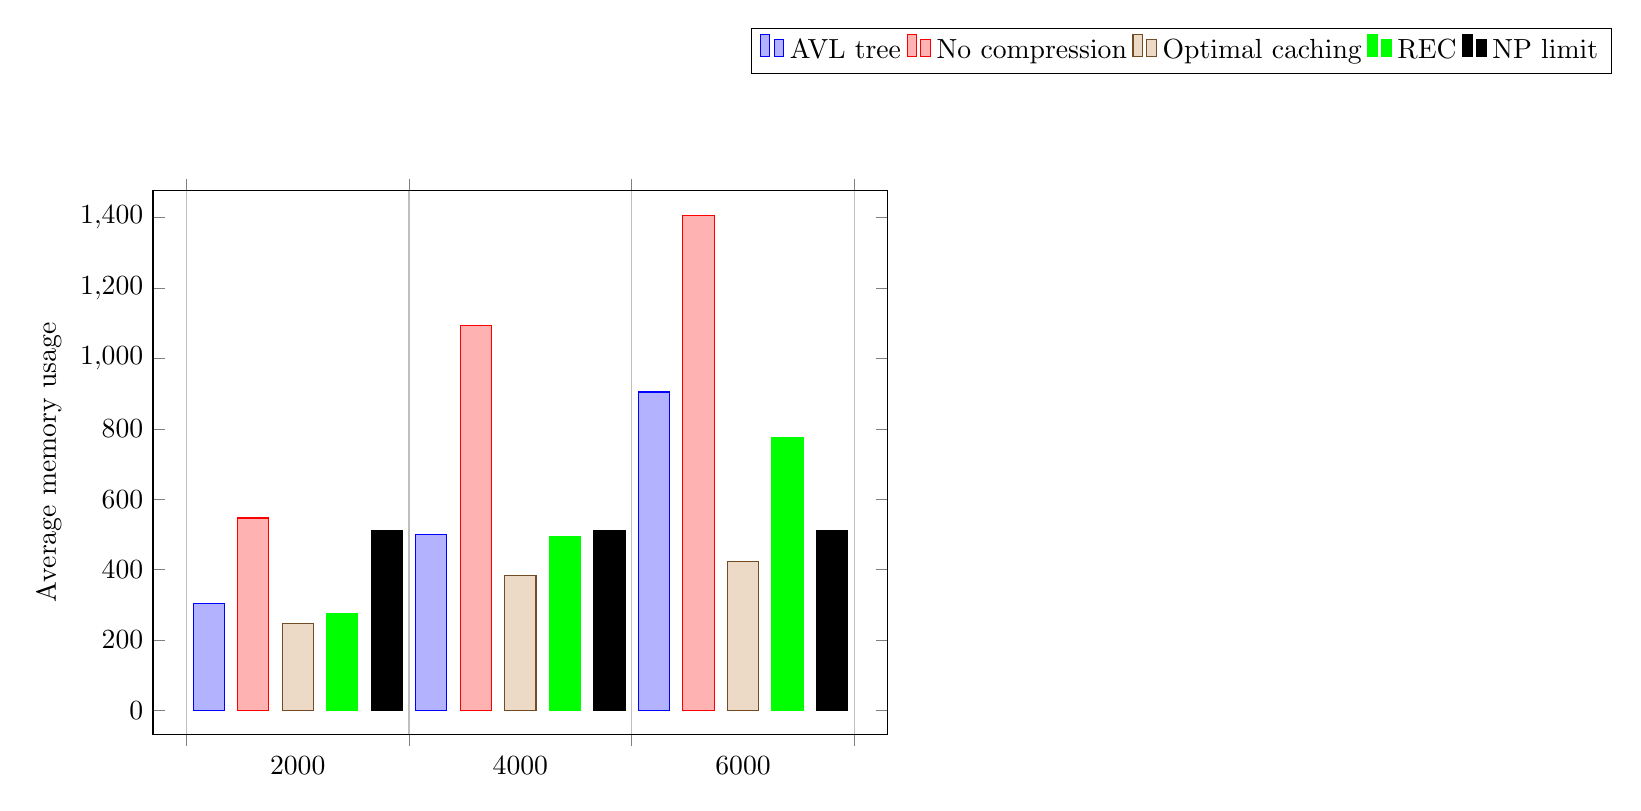
\begin{tikzpicture}
            \begin{axis}[
                width=0.9\linewidth,
                height=0.7\linewidth,
                %ylabel={Объём памяти [Кбайт]},
                %xlabel={Количество правил},
                %y label style={at={(-0.05, 0.5)}},
                %ymin=0, ymax=1700,
                %xmin=0, xmax=6500,
                %xmode=log,
                %log basis x={2},
                %xtick={1000, 2000, 3000, 4000, 5000, 6000},
                %ytick={0, 200, 400, 600, 800, 1000, 1200, 1400, 1600},
                %legend pos=north west,
                %ymajorgrids=true,
                %grid style=dashed,
                %cycle list name=color list
                x tick label style={
		            /pgf/number format/1000 sep=},
	            ylabel=Average memory usage,
	            enlargelimits=0.05,
	            legend style={at={(1.4, 1.3)},
	            anchor=north,legend columns=-1},
	            ybar interval=0.7,
                ] 
                \addplot+[] coordinates{(2000, 303.58)(4000, 500.58)(6000, 904.71)(8000, 1)};
                \addplot+[] coordinates{(2000, 546.58)(4000, 1093.58)(6000, 1406.25)(8000, 1)};
                \addplot+[] coordinates{(2000, 246.58)(4000, 382.58)(6000, 421.71)(8000, 1)};
                \addplot+[, color=green] coordinates{(2000, 273.58)(4000, 492.58)(6000, 773.71)(8000, 1)};
                \addplot+[mark=none, color=black] coordinates{(2000, 512)(4000, 512)(6000, 512)(8000, 1)};
                \legend{AVL tree, No compression, Optimal caching, REC, NP limit}
     
            \end{axis}
            \end{tikzpicture}
                \captionsetup{justification=centering}
                \caption{Network processor memory usage depends different flow table sizes.}
                \label{graph:compmem}
            %\end{adjustbox}
            \end{subfigure}
            \hfill
            \begin{subfigure}[b]{0.45\textwidth}
            %\begin{adjustbox}{width=\linewidth}
            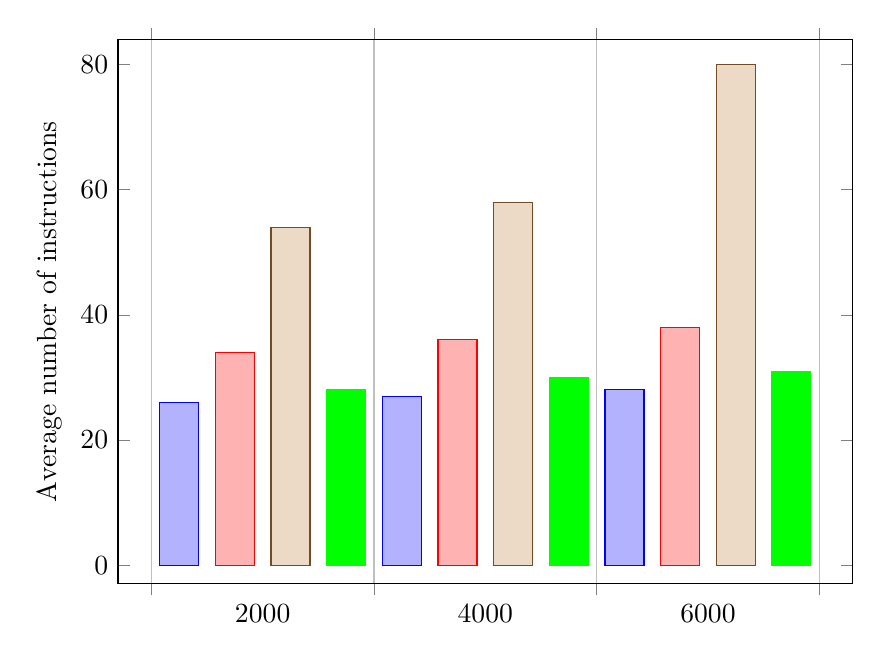
\begin{tikzpicture}
            \begin{axis}[
                width=0.9\linewidth,
                height=0.7\linewidth,
                %x tick label style={
		        %    /pgf/number format/1000 sep=}, 
                %ylabel={Среднее количество тактов},
                %xlabel={Количество правил},
                %y label style={at={(-0.05, 0.5)}},
                %ymin=0, ymax=90,
                %xmin=0, xmax=6500,
                %xmode=log,
                %log basis x={2},
                %xtick={1000, 2000, 3000, 4000, 5000, 6000},
                %ytick={0, 10, 20, 30, 40, 50, 60, 70, 80},
                %legend pos=north west,
                %ymajorgrids=true,
                %grid style=dashed,
                %cycle list name=color list
                x tick label style={
		            /pgf/number format/1000 sep=},
	            ylabel=Average number of instructions,
	            enlargelimits=0.05,
	            legend style={at={(0.5,-0.3)},
	            anchor=north,legend columns=-1},
	            ybar interval=0.7,
                ] 
                \addplot+[] coordinates{(2000,26)(4000,27)(6000,28)(8000, 1)};
                \addplot+[] coordinates{(2000,34)(4000,36)(6000,38)(8000, 1)};
                \addplot+[] coordinates{(2000,54)(4000,58)(6000,80)(8000, 1)};
                \addplot+[color=green] coordinates{(2000,28)(4000,30)(6000,31)(8000, 1)};
                \legend{}
                %\legend{АВЛ дерево, Без сжатия, Алгоритм ОК, Алгоритм REC}
     
            \end{axis}
            \end{tikzpicture}
                \captionsetup{justification=centering}
                \caption{Average number of instructions for processing one packet depends flow table size}
                \label{graph:compinst}
          %  \end{adjustbox}
            \end{subfigure}
        \end{figure*}

    \section{Future work}
        In the future works we will refine evaluation data. 
        We expect less memory usage with our compression algorithm implemented into flow table translator. 
        In the first experiments conducted, we obtained results showing a significant reduction in the amount 
        of memory usage with the help the data compression algorithm. After this we could check possibility 
        of TCAM memory implementation and use this compression algorithms for it.
    \section{Acknowledgements}
        This work is partially supported by the Russian Foundation for Basic Research under grant 19-07-01076.
\printbibliography{}
\end{document}
